\documentclass{article}
\usepackage{amsmath}
\usepackage{amssymb}
\usepackage{graphicx}
\usepackage{setspace}
\usepackage{subfigure}
\doublespacing
\title{Numerical Research on Gaussian Prime Cycles}
\author{Karen Dana \and Tyler Hardin}
\begin{document}
	\maketitle
	
A Gaussian integer is a complex number restricted to integer real and complex components. For example, 5+6i is a Gaussian integer, while 5.5+pi*I is not. A Gaussian prime, for the purposes of this paper, is a Gaussian integer such that one of the following is true
% https://tex.stackexchange.com/questions/114471/how-to-simply-center-equations-using-eqnarray
\begin{gather*}
  \mbox{im}(z) \mbox{ is prime and } \mbox{real}(z) = 0 \\
  \mbox{real}(z) \mbox{ is prime and } \mbox{im}(z) = 0 \\
  \sqrt{\mbox{real}(z)^2 + \mbox{im}(z)^2} \mbox{ is prime and } \mbox{real}(z) \neq 0 \mbox{ and } \mbox{im}(z) \neq 0
\end{gather*}
  
A Gaussian prime cycle, is a path formed by starting at an initial point, we will call $x_0$, with an initial direction (eg $(1,0)$), we will call d, and stepping right (that is $x_{n+1}=x_n + d$) until $x_n$ is a Gaussian prime. If $x_n$ is a Gaussian prime, we rotate $d$ $90^{\circ}$, and continue in that direction until another Gaussian prime is encountered; then we rotate again. This process continues until we return to our initial point and have our initial direction.

For our purposes, an equivalence relation is a relation that partitions a set. 
Equivalence classes are sets of elements that are all equal under a given equivalence relation. It is a known property of equivalence relations that every element belongs to exactly one class.
An example would be the natural numbers with the equivalence relation being equivalence modulus 2.
If $n$, a natural number, is even, it belongs to the class of even numbers which are all equal mod 2.
And vice versa if it is odd. Every number is either even or odd, so every number is in at least one class. No number is both even and odd, so no number can be in both classes. Thus every element is in exactly one class.
We use this concept to define an equivalence relation on the Gaussian prime cycles.
$G$, a Gaussian prime cycle, is considered equivalent to $H$, another Gaussian prime cycle, if $G$ can be rotated or translated such that the are the same shape.
More verbosely, they are equal if there exists a bijective translation-rotation transformation $T_M:G \to H$. \textit{Aside: Should I prove $T_M$ is an equivalence relation here?}

We plotted the number of classes in an initial point in a $l \times l$ grid as a function of $l$, with the grid being from $(0,0)$ to $(l-1,l-1)$ inclusively. Stated more simply: the number of unique shapes starting in the square and the size of the square. This allows us to see what the likely trend is as to the rate of discovering new shapes as one searches farther from $(0,0)$.

\begin{figure}[h!]
\centering
\includegraphics[scale=.5]{clgl30.png}
\caption{Number of classes as a function of grid size. Interestingly, the relation appears to be approximately linear.}
\end{figure}

We also plotted the length of a cycle as a (multi-valued) function of the distance from $(0,0)$. A trend in this would indicate that the farther one is from $0$, the longer the cycle one is likely to find. This was accomplished by plotting all cycles in a given grid for multiple grid sizes. Interestingly, the grouping and relative shape of the scatter plot is similar for many sizes of grid, even though the absolute difference is large.

\begin{figure}[h!]
\centering

\subfigure[All paths in grid of size $20$.]{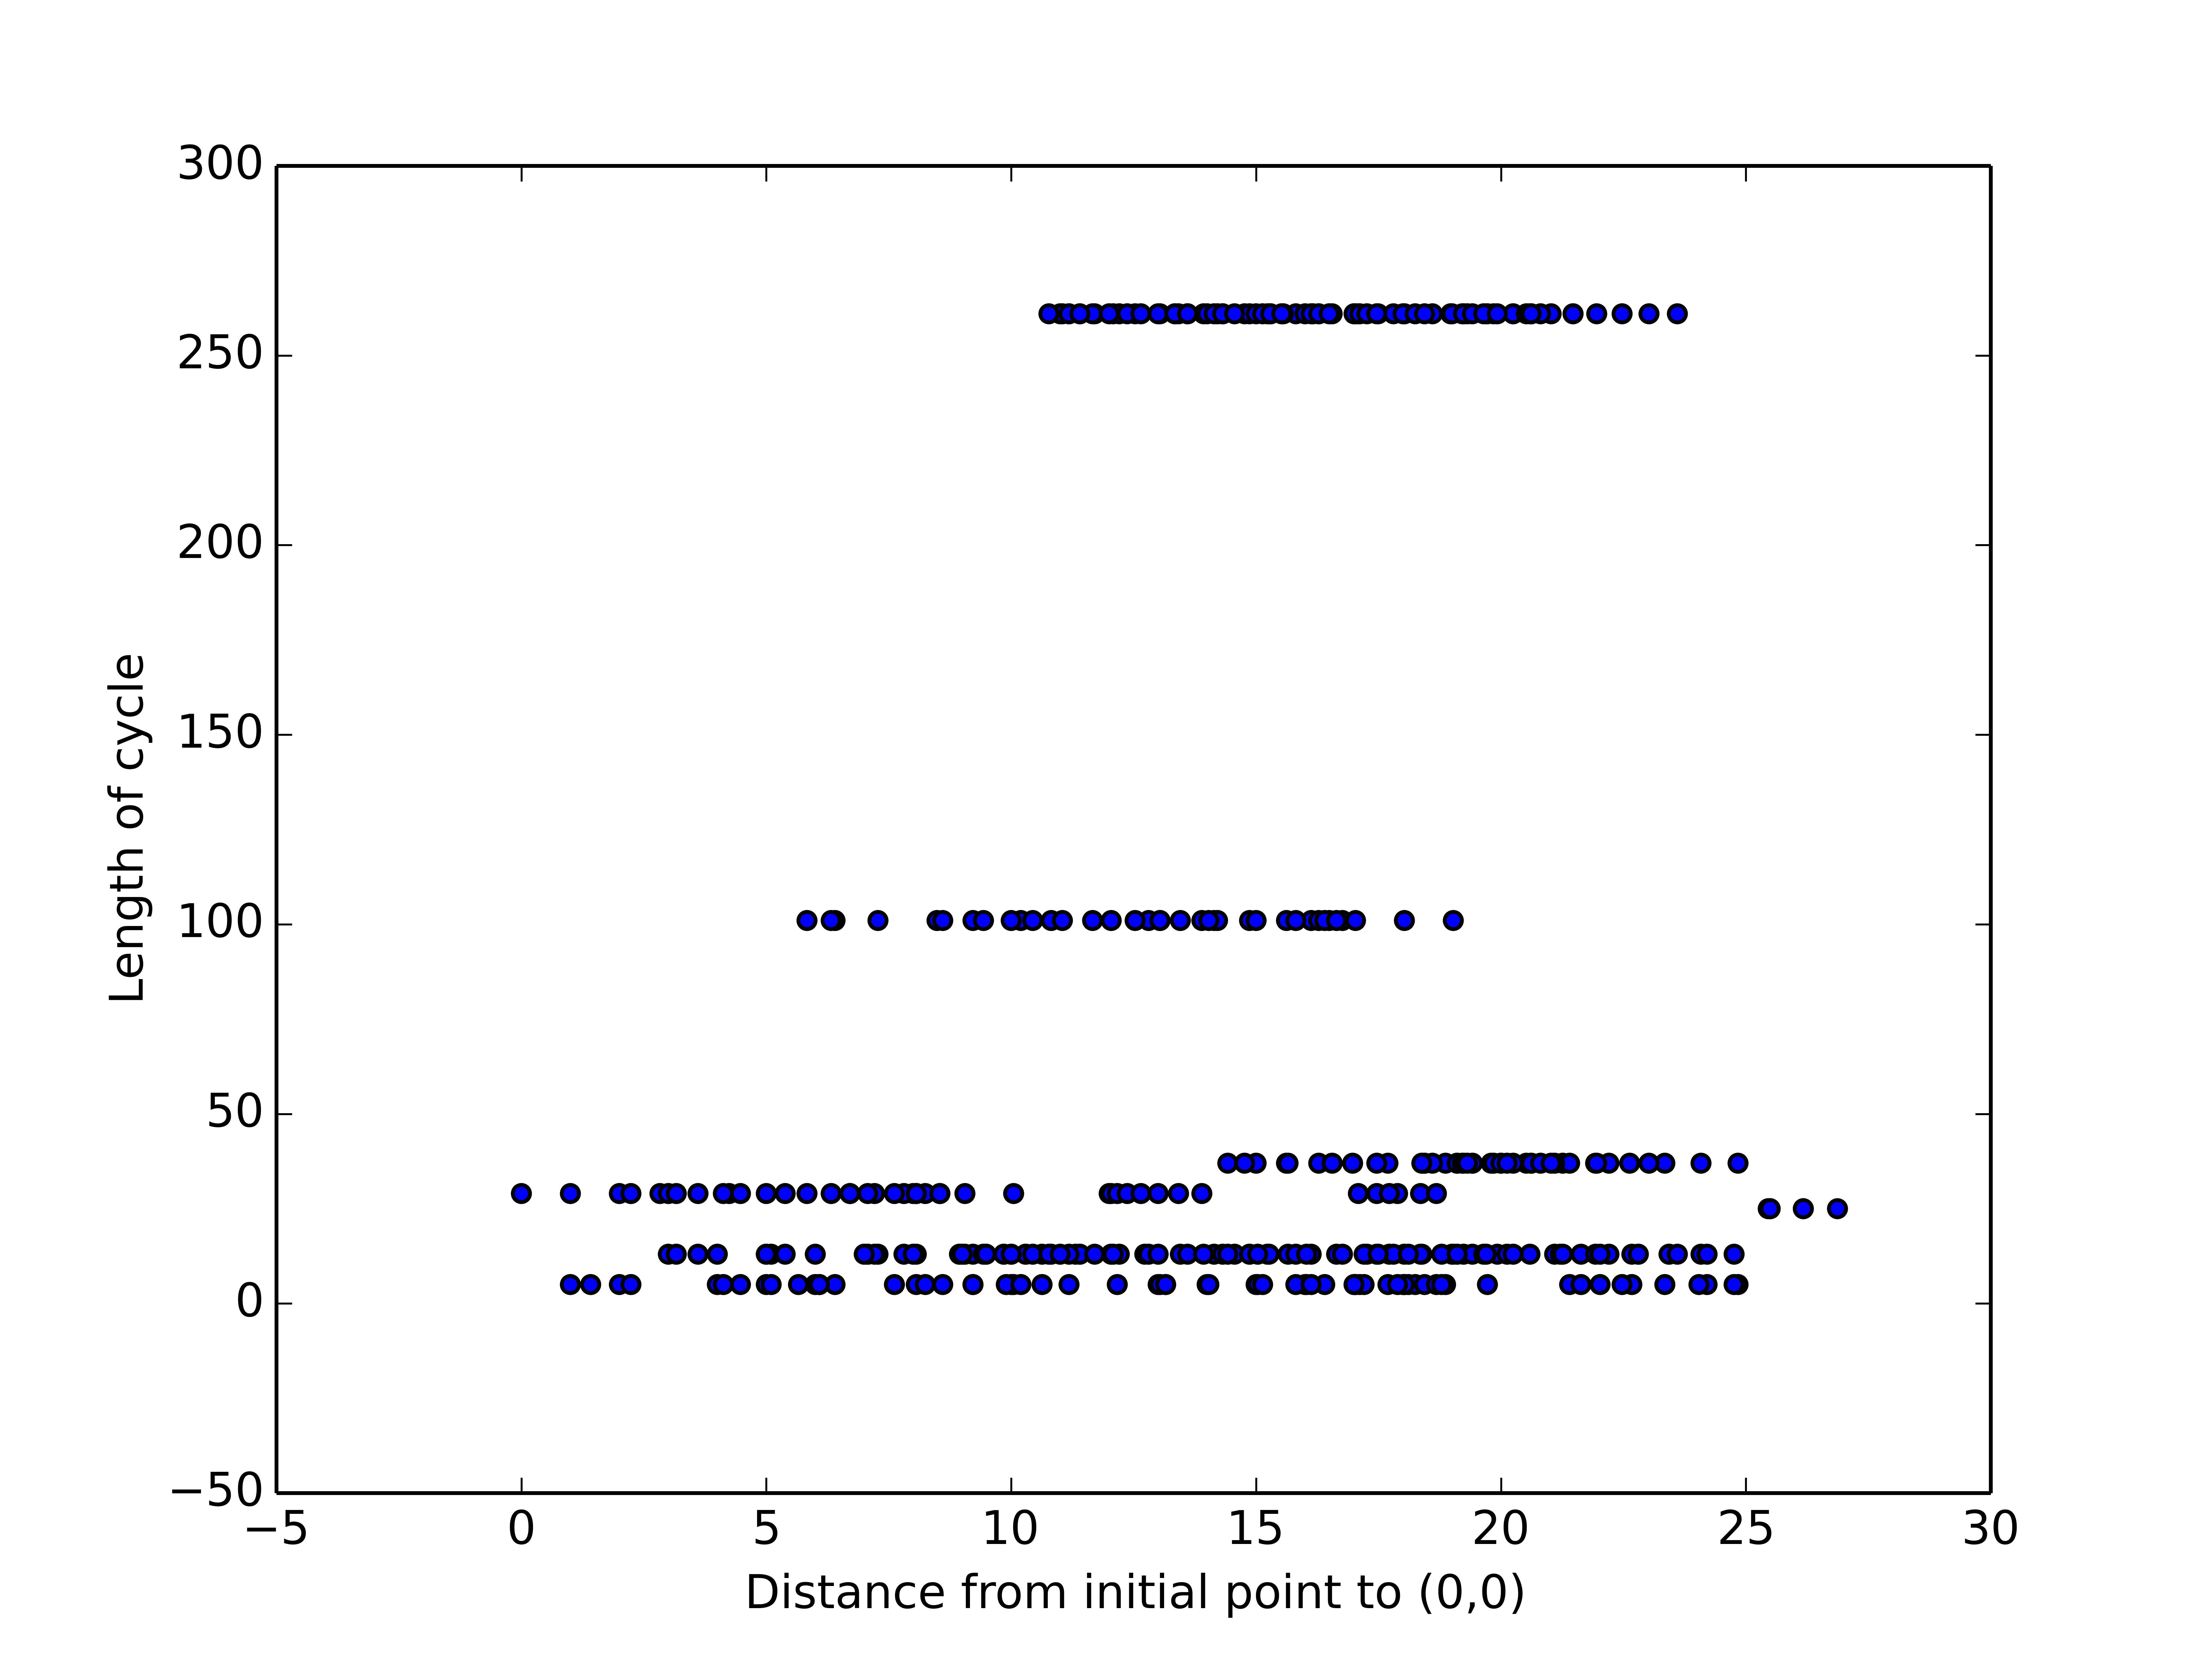
\includegraphics[scale=0.25]{icl20.png}}\\
\subfigure[All paths in grid of size $40$.]{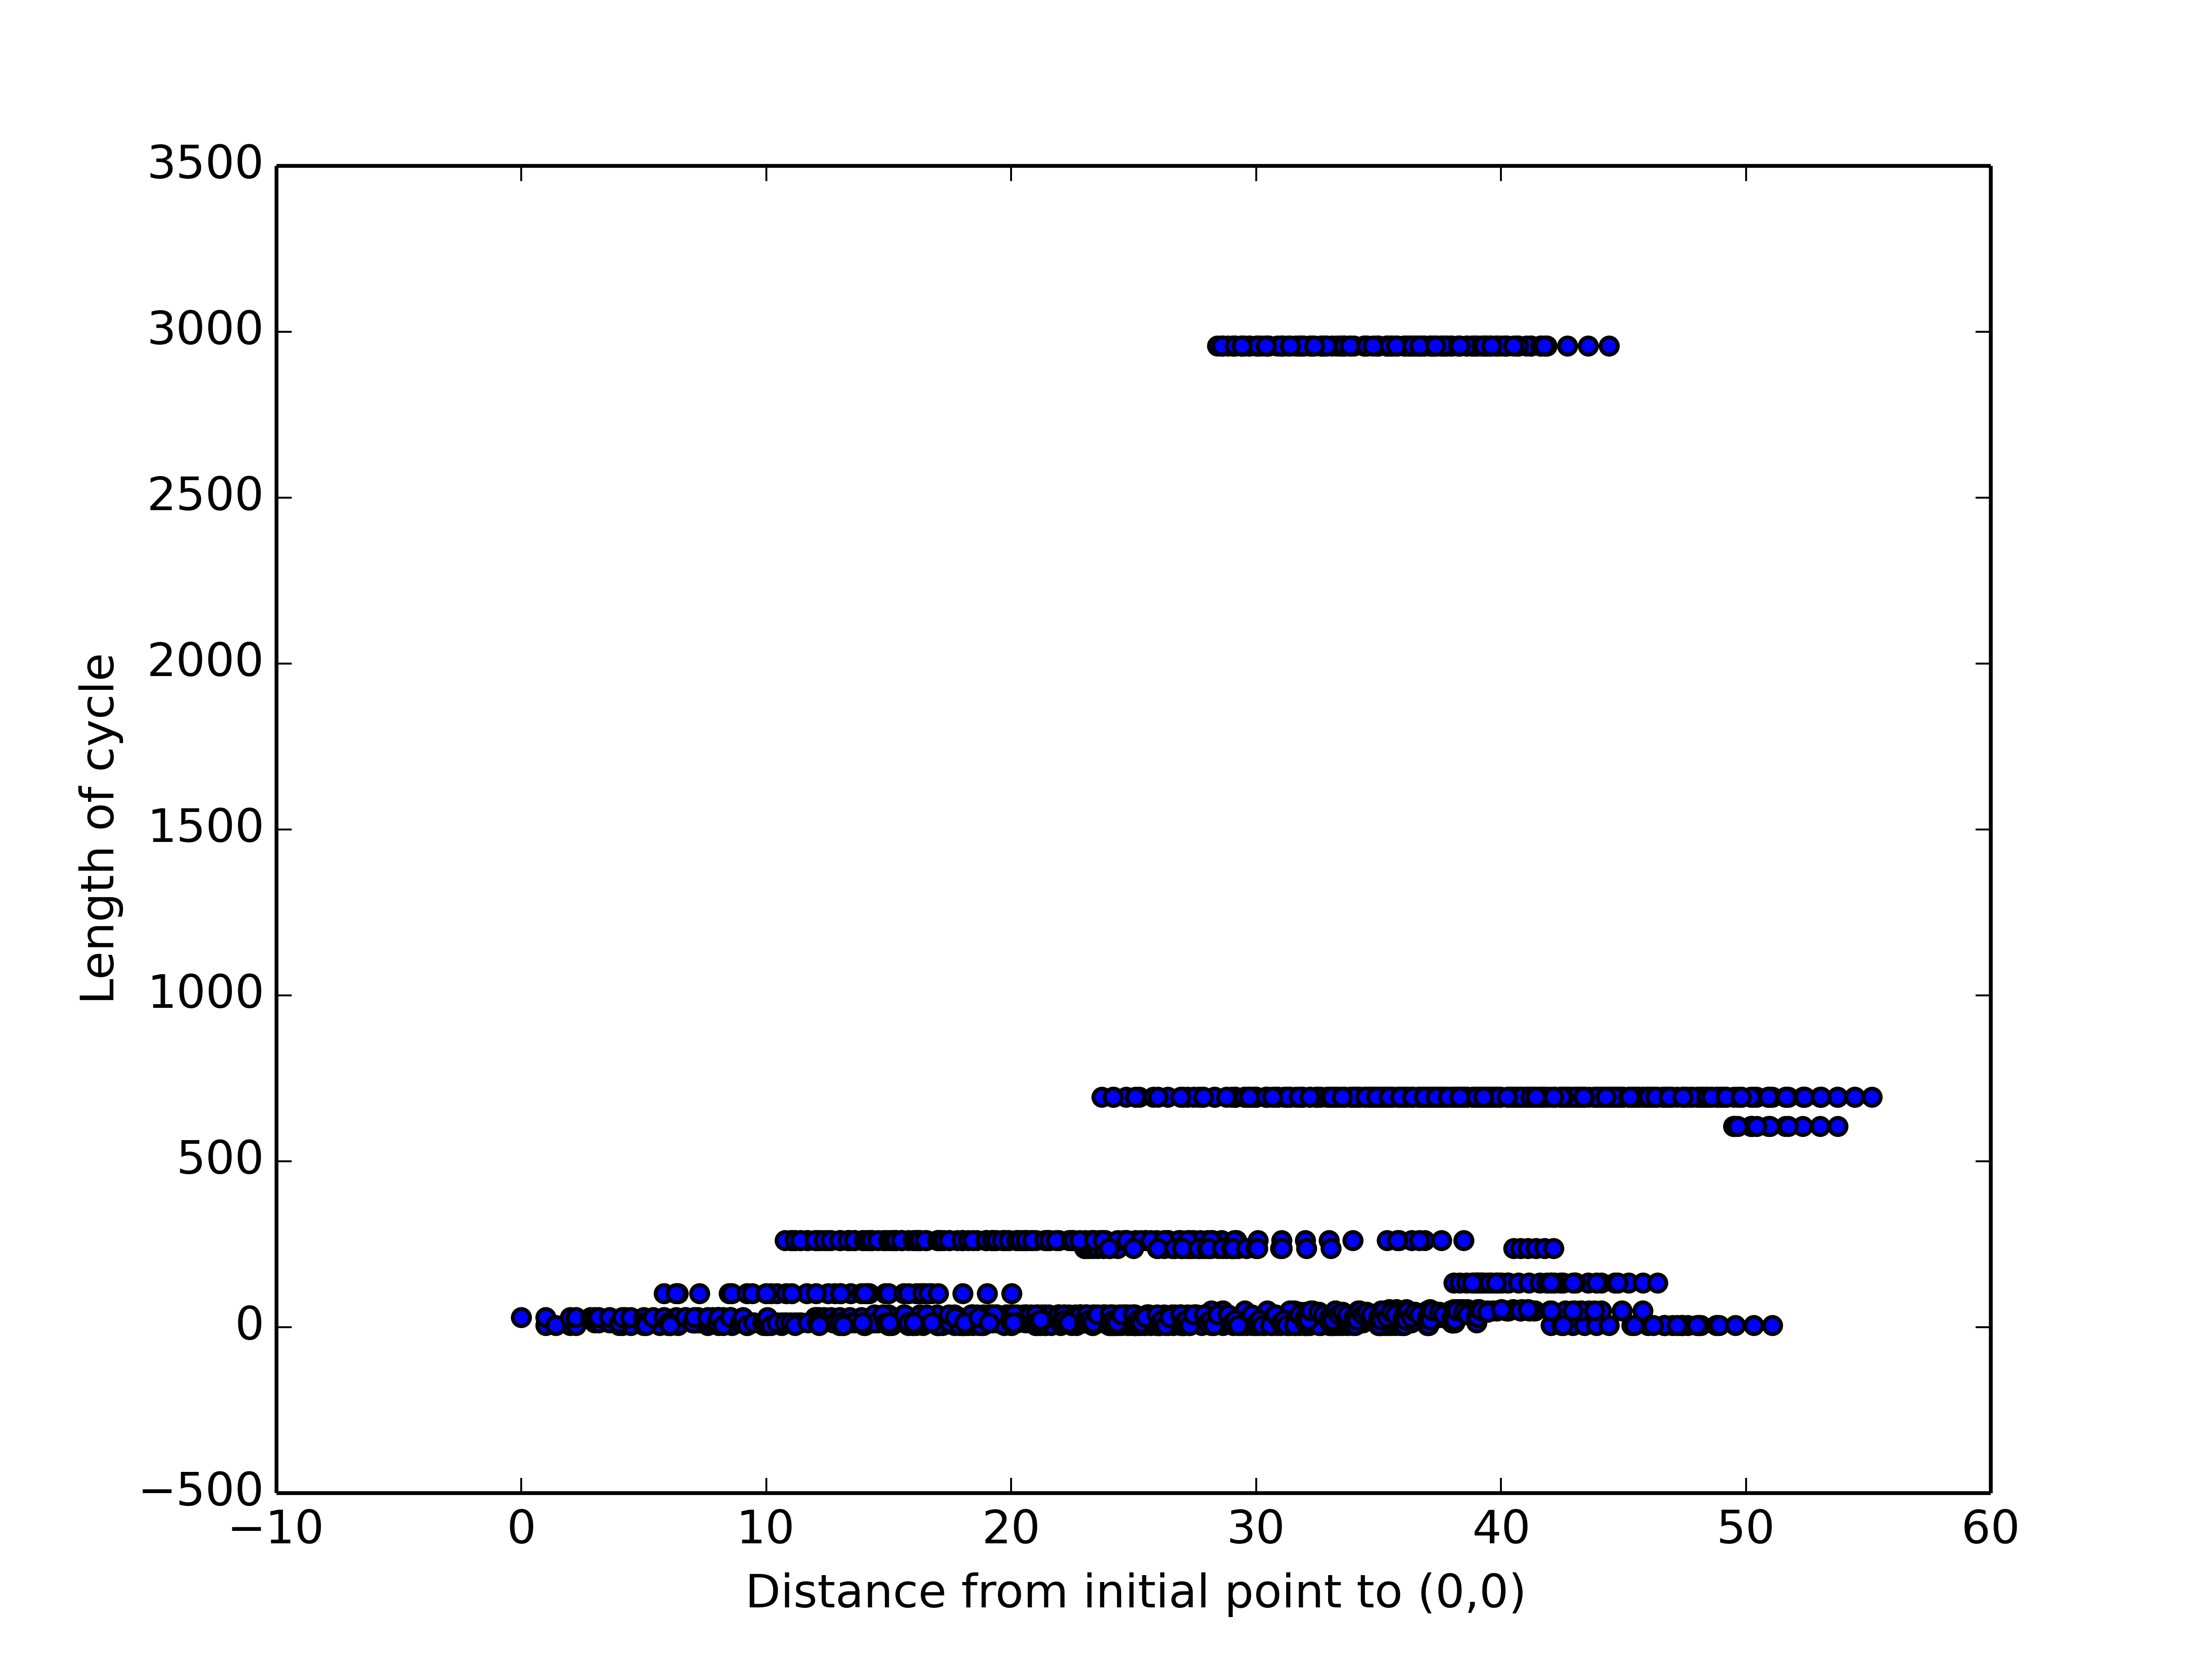
\includegraphics[scale=0.25]{icl40.png}}

\caption{Number of classes as a function of grid size. Notice how, in both, there are essentially three clusters.}
\end{figure}


\end{document}
